% Created 2020-10-13 Tue 13:28
% Intended LaTeX compiler: pdflatex
\documentclass[11pt]{article}
\usepackage[utf8]{inputenc}
\usepackage[T1]{fontenc}
\usepackage{graphicx}
\usepackage{grffile}
\usepackage{longtable}
\usepackage{wrapfig}
\usepackage{rotating}
\usepackage[normalem]{ulem}
\usepackage{amsmath}
\usepackage{textcomp}
\usepackage{amssymb}
\usepackage{capt-of}
\usepackage{hyperref}
\usepackage{amsthm}
\usepackage{url}
\newtheorem*{definition}{Definition}
\newtheorem*{example}{Example}
\newtheorem*{theorem}{Theorem}
\newtheorem*{exercise}{Exercise}
\newtheorem{question}{Question}
\usepackage[margin=1.25in]{geometry}
\usepackage{hyperref} % Required for adding links	and customizing them
\usepackage[dvipsnames]{xcolor}
\usepackage{booktabs}
\newcommand{\gr}{\textcolor{ForestGreen}}
\newcommand{\rd}{\textcolor{red}}
\newcommand{\R}{\mathbb{R}}
\newcommand{\frall}{\ \forall}
\author{Chris Ackerman}
\date{\today}
\title{Econ202A Notes}
\hypersetup{
 pdfauthor={Chris Ackerman},
 pdftitle={Econ202A Notes},
 pdfkeywords={},
 pdfsubject={},
 pdfcreator={Emacs 28.0.50 (Org mode 9.3)}, 
 pdflang={English}}
\begin{document}

\maketitle
\tableofcontents

\newpage

\section{Lecture 1---October 5, 2020}
\label{sec:orgbb91ca4}

Emphasis will be on neoclassical models of macroeconomic growth.

Office hours after class. Cohort effects are huge; spend lots of time collaborating with classmates. Start with certainty; converge to a single point steady state. With stochastic elements, we converge to a distribution. In both cases, we're studying an optimization problem. The model we're studying is the solution to an optimization problem. We will then discuss how to interpret these solutions as competitive equilibria. In these models, what is chosen by the planner and the competitive outcome are the same. In more realistic models, this won't be the case---there will be distortions. The goal is not to be theoretically rigorous; the focus is on applied macroeconomics---applying macroeconomic tools to study \textbf{the real world}. How can we use our theoretical models to interpret the real world or do interesting policy experiments?

\subsection{Basic Neoclassical Growth Model Cass-Koopmans)}
\label{sec:org65b7df6}
Economy consists of many identical infinitely lived households, each with the same preferences and endowments. There are several possible interpretations
\begin{itemize}
\item Representative Agent
\item Benevolent Social Planner
\item Infinitely Lived family
\end{itemize}
There is one production sector, and output is produced from capital and labor. Output can be either consumed or invested. There is only one type of output.

Investment becomes productive capital the following period:

\[
\max \sum^\infty_{t = 0} \beta^t u(c_t), \quad 0 < \beta < 0
\]
subject to

\begin{align*}
c_t + i_t \le y_t &= F(k_t, n_t) \tag{resource constraint}\\
k_{t + 1} &\le (1 - \delta)k_t + i_t, \quad 0 < \delta \le 1\\
0 \le n_t &\le 1\\
k &=\ \text{ given}
\end{align*}
Note that these are resource constraints, not budget constraints. They're different, and commonly confused. There are \emph{no prices} here! \(\delta\) is depreciation and \(\beta\) is a discount factor. The values for these terms are related to the length of time periods, \(t\).

We make some assumptions about the objects in our model. 

The production function \(F: \R^2_+ \to \R^+\) is

\begin{enumerate}
\item continuously differentiable
\item Homogeneous of degree  1 $\equiv$ constant returns to scale
\item Strictly quasi-concave
\item \begin{align*}
      F(0, n) &= 0 \tag{capital is essential}\\
F_k &= \text{ marginal product of capital}\\
&> 0 \\
F_n &> 0 \tag{ marginal product of labor }\\
 \end{align*}
\item INADA conditions
\[
\lim_{k \to 0} F_k(k, 1) = \infty \quad \lim_{k \to \infty} F_k(k, 1) = 0
\]
\end{enumerate}

The utility function \(u: \R_+ \to \R\) is
\begin{itemize}
\item Bounded---important for dynamic programming
\item Continuously differentiable
\item Strictly concave
\item $\lim_{c \to 0} u'(c) = \infty$
\end{itemize}

\textbf{Note}: We will use functional forms for \(F\) and \(u\) for almost everything in this class.

We make a few assumptions to simply the planners problem:
\begin{enumerate}
\item $F_n > 0 \implies n_t = 1$ for all $t$ and $u'(c) > 0$. We will introduce leisure in the utility function later.
\item $u'(c) > 0 \implies$ the resource constraint holds with equality,
\[
c_t + i_t = F(k_t, n_t)
\]
\item $\beta < 1 \implies$ a positive rate of return from giving up consumption today for consumption tomorrow; (actually $MP_k + 1 - \delta$)
\[
\implies k_t + 1 = (1 - \delta) k_t + i_t
\] 
\item Let
\[
f(k) \equiv F(k, 1) + (1 - \delta)k
\]
\end{enumerate}
We can now rewrite this problem as choosing a sequence of capital of stocks:
\begin{align*}
\max_{\{k_{t + 1}\}^\infty_{t = 0}}&\ \sum^\infty_{t = 0} \beta^t u(f(k_t) - k_{t +1})\\
0 \le k_{t + 1} &\le f(k_t)
\end{align*}
where \(k_0\) is given.
\begin{itemize}
\item This is called a "sequence problem" by Stokey and Lucas
\item There are infinitely many choice variables, so this problem is very hard to solve.
\item Instead we can use dynamic programming. We will solve the problem recursively, and therefore there's only one choice variable (next period's capital).
\end{itemize}

\subsection{Dynamic Programming}
\label{sec:org3bf10a5}

\begin{align*}
\intertext{Let }
V(k_0) &\equiv \max_{\{k_{t+1}\}{t = 0}^\infty} \sum^\infty_{t = 0} \beta^t u(f(k_t) - k_{t + 1})\\
\intertext{given $k_0$. We are maximizing the discounted utility given $k_0$. Rewrite as}
V(k_0) &= \max_{\{k_{t+1}\}_{t = 0}^\infty} \left\{ u(f(k_0) - k_1) + \beta \sum^\infty_{t = 1} \beta^{t - 1} u(f(k_t) - k_{t + 1})\right\}\\
&= \max_{k_1} \{u(f(k_0) - k_1) + \beta V (k_1)\}\\
\intertext{where}
V(k_1) &= \max_{\{k_{t + 1}\}^\infty_{t = 1}} \sum^\infty_{t = 1}\beta^{t - 1} u(f(k_t) - k_{t + 1})
\end{align*}

\subsubsection{Bellman's Equation}
\label{sec:org6125617}

\[
V(k) = \max_{k'} \left\{ u(f(k) - k') + \beta V(k')\right\}
\]
This is a functional equation where the unknown is \(V(k)\). \(V(k)\) is called the \emph{value function}. \(u(f(k) - k')\) is called the ``return function''. Our First Order Condition is
\[
u'(f(k) - k') = \beta V'(k').
\]
We want to solve for
\[
k' = g(k),
\]
which is the \emph{policy function}, often called the \emph{optimal policy function} or \emph{decision rule}. Later we'll prove that we can take FOCs because the function is differentiable.


\subsubsection{Solving for \(V(k)\)}
\label{sec:orgef52f58}
\begin{enumerate}
\item Guess a function $V_0(k)$.
\item Create a new function by applying a mapping to $V_0(k)$. We apply the operator $T$, so the new function is
\[
T(v_0(k)) = \max_{k'} \left\{u(f(k) - k') +_ \beta V_0(k')\right\}
\]
\item Let 
\[
V_1(k) = T(V_0(k))
\]
\item Repeat, forming a sequence of functions where 
\[
V_n(k) = T(V_{n - 1}(k)),
\]
creating (with a computer) the sequence $\{V_n\}^\infty_{n = 0}$, where each $V_n$ is a function.
\item Continue creating functions until $V_{n - 1}(k)$ and $V_n(k)$ are the same, or close enough for the desired error term.
\end{enumerate}
It turns out that this sequence is a Cauchy sequence, so we're guaranteed to get solutions that are arbitrarily close together. Look up contraction mappings, etc.

\section{Lecture 2---October 7, 2020}
\label{sec:org5fbb747}
The \(T\) we discussed yesterday is known as the \emph{Bellman Operator}.


Very few cases exists where we can fin a fixed point analytically. We can find a fixed point analytically when the return function is quadratic and the constraints are linear. If a closed form exists, we can find it use the \emph{method of undetermined coefficients}. This is Problem 1 in our homework, and involves two steps.

\begin{enumerate}
\item Find the functional form for $V$. For example, if $V_n(k)$ is quadratic and $T(V_n(k))$ is quadratic, $V(k)$ must be quadratic.
\item Find the parameter of the fixed point.
\end{enumerate}

If the operator takes in a quadratic function and outputs a quadratic function, we know the limit must be a quadratic function, so we can guess a quadratic solution and find the parameters. For the homework, think about log-linear functional forms.

\begin{example}
Suppose
\[
V_n(k) = ak^2 + bk + c
\]
and
\[
T(V_n(k)) = \tilde{a}k^2 + \tilde{b}k + c.
\]
$T$ transofrms a quadratic function into another quadratic function, so the fixed point is a quadratic function. How do we find the fixed point? It must be the case that
\begin{align*}
\tilde{a} &= f_1(a, b, c)\\
\tilde{b} &= f_2(a, b, c)\\
\tilde{c} &= f_3(a, b, c)\\
\end{align*}
Now we're solving a system of three equations in three unknowns. How do we know if $v$ (the fixed point) exists and is unique? We will use a few concepts from Stokey and Lucas, Chapter 3.
\end{example}

\begin{theorem}[Contraction Mapping Theorem]
If $(S, \rho)$ is a complete metric space and $T: S \to S$ is a contraction mapping with modulus $\beta$, then
\begin{enumerate}
\item $T$ has exactly one fixed point $V \in S$, and
\item for any $v_0 \in S$, $\rho(T^nV_0, V) \le \beta^n \rho (V_0, V)$ for $n = 0, 1, 2 \ldots$
\end{enumerate}
\end{theorem}
Since we've defined \(\beta\) such that \(0 \le \beta < 1\), we can get arbitrarily close to the fixed point by sending \(n \to \infty\).

\begin{itemize}
\item $S$ is a sequence of functions
\item $\rho$ is a measure of distance between two points in $S$ (a metric)
\item A Cauchy sequence is a sequence $\{V_n\}^\infty_{n = 1}$ of elements of $S$ where, for all $\varepsilon > 0$, there exists $N_\varepsilon$ such that $\rho(V_n, V_m) < \varepsilon$ for all $n, m > N_\varepsilon$.
\item Complete---every Cauchy sequence in $S$ converges to some element of $S$.
\end{itemize}

\begin{definition}[Contraction Mapping]
A \gr{contraction mapping} $T: S \to S$ is a contraction if, for some $\beta \in (0, 1)$,
\[
\rho(Tx, Ty) \le \beta \rho(x, y)
\]
for any $x, y \in S$.
\end{definition}

A \gr{fixed point} is some \(v \in S\) such that \(Tv = v\).

\textbf{Problem}: While the theorem guarantees that iterating on Bellman's equation will provide a sequence of functions that converges to a unique fixed point, verifying the conditions of the theorem is hard.

\begin{theorem}[Blackwell's Sufficient Condition for a Contraction]
Let $X \subseteq \R^n$ and $B(X)$ be a space of \underline{bounded functions} $f: X \to \R$ with the $\sup$ norm, $\|f\| = \sup_x |f(x)|$. Let $T: B(x) \to B(x)$ satisfy
\begin{enumerate}
\item 
\[
f, g \in B(x) \land f(x) \le g(x) \frall x \in X \implies (Tf)(x) \le (Tg)(x) \frall x \in X \tag{monotonicity}
\]
In words, if we have two functions that satisfy the initial assumption on the left, the Bellman operator preserves this ordering.
\item There exists some $\beta \in (0, 1)$ such that 
\[
[T(f + a)](x) \le (Tf)(x) + \beta a \tag{discounting}
\]
for all $f \in B(X)$ and $a \ge 0$.
\end{enumerate}
\end{theorem}

Intuitively, \(T\) is the sum of two functions: the current return and the future return. We need these functions to get closer and closer to a fixed point. It is sufficient to replace a general bounded function with this scalar and then show that this is a contraction.

\begin{exercise}
Verify that the Bellman mapping
\[
T: B(X) \to B(X)
\]
from the neoclassical growth model satisfies monotonicity and discounting.
\end{exercise}

\subsection{Envelope Condition and Euler Equation}
\label{sec:org357e618}
The FOC for the right hand side of the Bellman equation is
\[
u'(f(k) - g(k)) = \beta V'(g(k)),
\]
where \(k' = g(k)\). The goal here is to go from our sequence problem to the Euler equation. We can get the Euler equation FOC directly by taking derivatives of the sequence problem. Note that the Bellman operator maps concave functions to concave functions.

\begin{theorem}[Envelope Theorem]
Suppose $v$ is concave and $w$ is concave and differentiable with
\[
w(x_0) = v(x_0) \text{ and } w(x) \le v(x)
\]
for all $x$ in a neighborhood of $x_0$. Then $v$ is differentiable at $x_0$ and
\[
v_i (x_0) = w_i (x_0).
\]
\end{theorem}
\(v\) is a function we don't necessarily know, but we know it is concave. \(w\) is a function we are going to make up. We want it to be concave and differentiable, and we want the two functions to be exactly the same at \(x_0\). If we form \(w\) this way, we know we can take its derivative, since we designed it to be differentiable. If we take the \(i^{\text{th}}\) partial of \(w\) and evaluate it at \(x_0\), then its \(i^{\text{th}}\) partial derivative is exactly the same as the \(i^{\text{th}}\) partial of \(v\). In the case of the Bellman mapping, let
\begin{align*}
w(k) &\equiv u(f(k) - g(k_0)) + \beta V(g(k_0))\\
\implies w(k_0) &= (k_0)\\
w(k) &\le v(k) \text{ for } k \text{ near } k_0.
\end{align*}
Intuitively, we're holding the future fixed and the only thing that's moving is the current capital stock. We only require this condition to hold locally; the picture below is a zoomed-in version of the Envelope Theorem. We aren't assuming anything about the behavior of either of these functions anywhere else.

\begin{center}
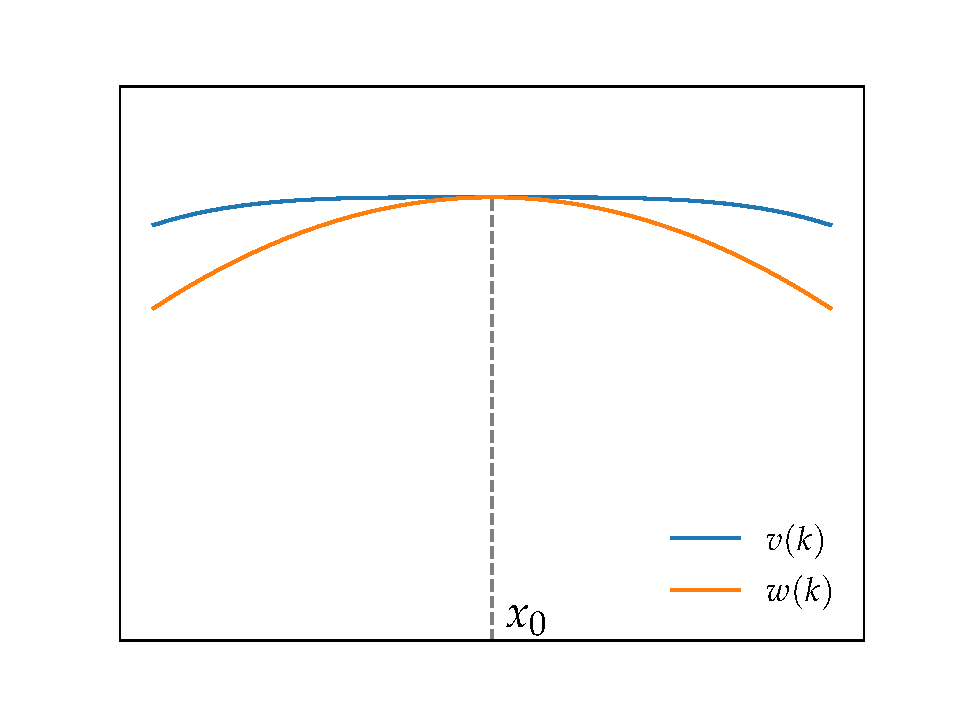
\includegraphics[width=0.75\textwidth, keepaspectratio=true]{figures/envelope_theorem.pdf}
\end{center}

\begin{definition}[Envelope Condition]
\[
V'(k_0) = w'(k_0) = u'(f(k_0) - g(k_0))f'(k_0) \tag{chain rule}
\]
in general,
\[
v'(k) = u'(f(k) - g(k))f'(k).
\]
We can characterize the derivative of the value function without knowing the value function. Combine these two equations, and we get
\[
u'(f(k) - g(k)) = \beta u'(f(g(k)) - g(g(k)))f'(g(k))
\]
or
\[
u'(f(k_t) - k_{t + 1}) = \beta u'(f(k_{t + 1}) - k_{t + 2})f'(k_{t + 1}). 
\]
This is the Euler Equation. The RHS is discounting the marginal utility of capital from next period. $\beta$ is discounting, and $u'$ is the marginal utility of capital.
\end{definition}
It is important that \(k\) doesn't appear by itself (will show up later in class).

\rd{REVIEW TWO WAYS TO OBTAIN EULER EQUATION}

Intuition for \(f'(k_{t + 1})\): \(f(k_{t + 1})\) is the output we can produce next period. \(f'\) is the derivative of that production function, and we can think of it as the slope of the production function, or the (limit of) additional output we get divided by the additional capital deployed. \(u'\) is the additional utility we get from an additional amount of consumption.

There is only one \(k_1\) that will give a sequence, from the Euler equation, that satisfies the \emph{transversality condition}. We have one Euler equation for each \(t \ge 0\), so\ldots infinitely many. This isn't good, since we have too many equations! But the Bellman equation doesn't have this problem. How can we get a similar solution for the Euler equations?

\begin{definition}[Transversality Condition]
\[
\lim_{t \to \infty} \beta^t u'(f(k_t) - k_{t + 1}) f'(k_t) \cdot k_t = 0
\]
Working from right to left, this limit is the capital stock, multiplied by the marginal product of capital. Now we want to turn this into utility, so we multiply it by the utility of the output produced from this stock of capital. Finally, we have to discount this back to today, since this is future output/utility. Intuitively, this whole term is the present value of capital that we have in period $t$. As we send the limit to infinity, our future capital is worth nothing. Using this condition allows us to pin down the infinite sequence from the Euler equations. If we choose an arbitrary $k_1$ instead, we can end up with either negative consumption or a negative capital stock, neither of which makes sense. \rd{VERIFY THIS NUMERICALLY}. Mathematically, there is only one $k_1$ that lies on the saddle path.
\end{definition}

\begin{theorem}[Sufficiency of the Euler and transversality conditions; Stokey and Lucas 4.15]
Let $X \subset \R^l_+$, and let $F$ satisfy the following conditions:
\begin{enumerate}
\item $X$ is a convex subset of $\R^l$, and the correspondence $\Gamma: X \to X $ is non-empty, compact-valued, and continuous.
\item The function $F: A \to \R$ is bounded and continuous, and $0 < \beta < 1$.
\item For each $y$, $F(\cdot, y)$ is strictly increasing in each of its first $l$ arguments.
\item $F$ is strictly concave.
\item $F$ is continuously differentiable on the interior of $A$.
\end{enumerate}
Then the sequence
\[
\{x^*_{t + 1}\}^\infty_{t = 0}, \text{ with } x^*_{t + 1} \in \operatorname{int} \Gamma (x^*_t), t = 0, 1, \ldots
\]
is optimal for the problem
\begin{align*}
\sup_{\{x_{t + 1}\}^\infty_{t = 0}} \sum^\infty_{t = 0} & \beta^t F(x_t, x_{t + 1})\\ 
\text{s.t. } x_{t + 1} &\in \Gamma(x_t), t = 0, 1, 2,\ldots,\tag{SP}\label{SP}\\
\text{given } x_0 & \in X
\end{align*}
if the sequence satisfies
\begin{align*}
0 &= F_y(x_t^\ast, x_{t + 1}^\ast) + \beta F_x(x_{t + 1}^\ast, x_{t + 2}^\ast), \quad t = 0, 1, 2,\ldots\tag{2}\label{LS4.15:2}\\
0 &= \lim_{t \to \infty} \beta^t F_x(x_t^\ast, x_{t + 1}^\ast) \cdot x_t^\ast \tag{3}\label{LS4.15:3}
\end{align*}
\end{theorem}
\begin{proof}
Take $x_0$ as given, assume $\{x_t^\ast\} \in \Pi(x_0)$ satisfies \ref{LS4.15:2} and \ref{LS4.15:3}, and let $\{x_t\} \in \Pi(x_0)$ be any feasible sequence. It is sufficient to show that the difference (call it $D$) between the objective function in \ref{SP} evaluated at $\{x_t^\ast\}$ and $\{x_t\}$ is nonnegative.
\begin{align*}
\intertext{Since $F$ is continuous, concave, and differentiable,}
D &= \lim_{T \to \infty} \sum^T_{t = 0}\beta^t [F(x_t^\ast, x_{t + 1}^\ast) - F(x_t, x_{t + 1})]\\
&\ge \lim_{T \to \infty} \sum^T_{t = 0} \beta^t[F_x(x_t^\ast, x_{t + 1}^\ast)\cdot (x_t^\ast - x_t) + F_y(x_t^\ast, x_{t + 1}^\ast)\cdot (x_{t + 1}^\ast - x_{t+ 1})].\\
\intertext{Since $x_0^\ast - x_0 = 0$, rearranging terms gives}
D &\ge \lim_{T \to \infty}\left\{\sum^{T - 1}_{t = 0} \beta^t[F_y(x_t^\ast, x_{t+1}^\ast) + \beta F_x(x_{t + 1}^\ast, x_{t + 2}^\ast)]\cdot (x_{t + 1}^\ast - x_{t + 1}) + \beta^T F_y (x_T^\ast, x_{T + 1}^\ast)\cdot(x_{T + 1}^\ast - x_{T + 1})\right\}.\\
\intertext{Since $\{x_t^\ast\}$ satisfies \ref{LS4.15:2}, all the terms in the summation are zero. Substituting from \ref{LS4.15:2} into the last term and using \ref{LS4.15:3} gives}
D &\ge - \lim_{T \to \infty} \beta^T F_x(x_T^\ast, x_{T + 1}^\ast)\cdot (x_T^\ast - x_T)\\
&\ge - \lim_{T \to \infty} \beta^T F_x (x_T^\ast, x_{T + 1}^\ast) \cdot x_T^\ast.
\end{align*}
The last line uses the fact that $F_x \ge 0$ (one of our assumptions) and $x_t \ge 0$ for all $t$. It follows from \ref{LS4.15:2} that $D \ge 0$, establishing the desired result.
\end{proof}

\subsection{Things to know for exam/course}
\label{sec:org3bfe9eb}
\begin{enumerate}
\item Contraction mapping theorem
\item Won't be tested on complete metric space, Cauchy sequence; we'll be dealing with specific functional forms that meet our assumptions
\item We are expected to be able to verify the Blackwell Sufficient Conditions
\end{enumerate}

\section{TA Section---October 9, 2020 (Introduction to Dynamic Programming)}
\label{sec:org2058d9e}

\subsection{The Sequential Problem and its Solution}
\label{sec:org2a683c6}

Consider the simple deterministic neoclassical growth model. We don't have prices, just the resource constraint and the capital accumulation equation. We have an infinitely-lived household, so the utility function depends on a sequence of consumption and is time-separable,
\[
\sum^\infty_{t = 0} \overbrace{\beta^t}^{\text{discount factor}} \underbrace{u(c_t)}_{\text{instantaneous utility}}.
\]
The agent chooses a sequence of consumption, capital and investment,
\[
\{c_t, k_{t + 1}, i_t\}^\infty_{t = 0}
\]
subject to
\begin{align*}
c_t + i_t &\le \underbrace{F(k_t, n_t)}_{\text{predetermined output}} \tag{resource constraint}\\
k_{t + 1} &= i_t + \underbrace{(1 - \delta)k_t}_{\scriptsize{\begin{tabular}{c}undepreciated\\capital\end{tabular}}}]\tag{capital accumulation}\\
n_t &\in [0, 1] \tag{labor}\\
c_t, k_t &\ge 0 \frall t\tag{non-negativity constraints}\\
k_o &\text{ given}
\end{align*}

We can substite for investment in our initial problem to get
\[
c_t + \{k_{t + 1} - (1 - \delta) k_t\} = F_{t + 1}.
\]
We can further simplify this so that the only thing we're choosing is a sequence of capital levels. Assuming \(\delta = 1\), we get
\[
\max_{\{k_{t + 1}\}^\infty_{t = 0}} \sum^\infty_{t = 0} \beta^t \left(f(k_t) - k_{t + 1}\right)
\]
with \(0 \le k_{t + 1} \le f(k_t)\) and \(k_0\) given. We can now derive the Euler equation. There are only two terms that depend on \(k_{t + 1}\),
\[
\ldots \beta^t u(f(k_t) - f_{t + 1} + \beta^{t + 1} u(f(k_{t + 1}) - k_{t + 2}) \ldots
\]
Now we can take the derivative with respect to \(k_{t + 1}\),
\[
\beta^t u' (f(k_t) - k_{t + 1})\cdot -1 + \beta^{t + 1} u'(f(k_+{t + 1}) - k_{t + 2}) \cdot f'(k_{t + 1}).
\]
Simplifying,
\[
\underbrace{u'(f(k_t) - k_{t + 1})}_{c_t} = \beta \underbrace{f'(k_{t + 1})}_{\text{MP}k} \cdot u'(\underbrace{f(k_{t + 1}) - k_{t + 2}}_{c_{t + 1}}).
\]
In words, the marginal cost of forgone consumption today must be the same as the discounted value of tomorrow's marginal product of capital, plus the marginal utility from consuming tomorrow's output.

\subsection{Analytic Solution (full depreciation)}
\label{sec:orgd03de9d}

\begin{align*}
u(c) &= \log(c)\\
f(k) &= k^\alpha, \quad \alpha \in (0, 1)\\
u'(c) &= \frac{1}{c}\\
f'(k) &= \alpha k^{\alpha - 1}\\
(k_t^\alpha - k_{t + 1})^{-1} &= \beta \alpha k^{\alpha - 1}_{t + 1}(k^\alpha _{ t + 1} - k_{t + 2})^{-1}\tag{Euler Equation}\\
\implies k_{t + 1}^\alpha - k_{t + 2} &= \beta \alpha k_{t + 1}^{\alpha - 1}(k^\alpha_t - k_{k + 1})\\
\intertext{We want}
k_{t + 1} &= g(\underbrace{k_t}_{\text{given}}).\\
\intertext{The limit of the solution to the finite horizon problem is equivalent to the unique solution to the infinite horizon problem.} 
k^\alpha_{t + 1} - k_{t + 2} &= \beta \alpha k^{\alpha - 1}_{t + 1} (k^\alpha_t - k_{t + 1}) \text{ for } t = 1, 2, \ldots , T - 1.\\
\intertext{We have $\underbrace{k_0}_{\text{given}}, k_1, \ldots, K_T$. This leaves us $T$ variables and $T - 1$ equations, so we need to consider the terminal condition,}
\underbrace{\beta^t u'(c_T)}_{> 0} \cdot k_{T + 1} &= 0\\
\implies k_{T + 1} &= 0.\\
\intertext{Consider the Euler Equation for $t = T - 1$,}
k^\alpha_T - k_{T + 1} &= \beta \alpha k_T^{\alpha - 1}(k^\alpha_{T - 1} - k_t)\\
k^\alpha_T &= \beta \alpha k_T^{\alpha - 1}(k^\alpha_{T - 1} - k_T)\\
k_T &= \beta \alpha (k^\alpha_{T - 1} - k_T)\\
\implies k_T &= \frac{\beta \alpha}{1 + \beta \alpha} k^\alpha_{T - 1}\\
\intertext{Iterate on $t = T - 2$,}
k_{T - 1} &= \frac{\alpha \beta (1 - \alpha \beta)}{(1 + \alpha \beta + (\alpha \beta)^2)}k_{T - 2}\\
\intertext{Taking the limit as $t \to \infty$,}
k_{t + 1} &= \frac{\alpha \beta (1 - (\alpha \beta)^{T _ t})}{1 - (\alpha \beta)^{T - t + 1}} k^\alpha_t\\
k_{t + 1} &= \alpha \beta k_t^\alpha.
\intertext{The intuition is that}
\text{savings } &= \text{ investment}\\
&= \alpha \beta k_t^\alpha\\
s/y &= \alpha \beta\\
\text{consumption } &= (1 - \alpha \beta)k^\alpha_t. 
\end{align*}

\subsection{The Recursive Problem and its Solution}
\label{sec:orgdd67d09}
Define a real-valued function \(V(k)\),
\begin{align*}
V(k_0) &= \max_{\left\{k_{t + 1}\right\}^\infty_{t = 0}} \sum^\infty_{t = 0} \beta^t u(f(k_t) - k_{t + 1})\\
\text{s.t. } 0 &\le k_{t + 1} \le f(k_t)\\
\text{given } &k_0\\
\intertext{We want}
V(k_0) &= \text{Return } + \beta \cdot V(k_1).\\
V(k_0) &= \max_{k_1} \max_{\left\{k_{t + 1}\right\}^\infty_{t = 1}} \sum^\infty_{t = 0} \beta^t u(f(k_t) - k_{t + 1})\\
V(k_0) &= \max_{k_1} \max_{\left\{k_{t + 1}\right\}^\infty_{t = 1}} u (f(k_0) - k_1) + \beta u(f(k_1) - k_2) + \ldots\\
V(k_0) &= \max_{k_1} \max_{\left\{k_{t + 1}\right\}^\infty_{t = 1}} \beta u(f(k_0) - k_1) + \beta \sum^\infty_{t = 1} \beta^t \cdot u(f(k_1) - k_{t + 1})\\
V(k_0) &= \max_{k_1} \beta u(f(k_0) - k_1) + \underbrace{\max_{\left\{k_{t + 1}\right\}^\infty_{t = 1}} \beta u(f(k_0) - k_1) + \beta \sum^\infty_{t = 1} \beta^t \cdot u(f(k_1) - k_{t + 1})}_{\beta \max_{\{k_{t + 1}\}^\infty_{t = 1}} \sum^\infty_{t = 1} u(f(k_t) - k_{t + 1})}\\
V(k_0) &= \max_{k_1} u(f(k_0) - k_1) + \beta V(k_1)\\
V(k) &= \max_{k_1} u(f(k) - k') + \beta V(k')\\
\intertext{Where $k'$ denotes tomorrow's capital stock. The optimal $k'$ is}
0 &= -1\cdot u'(f(k) - k') + \beta V'(k') \\
u'(f(k) - k') &= \beta V'(k')\\
\intertext{Suppose}
V(k) &= A + \frac{\alpha}{1 - \alpha \beta} \ln(k)\\
V'(k) &= \frac{\alpha}{1 - \alpha \beta}\cdot k^{-1}\\
V'(k') &= \frac{\alpha}{1 - \alpha \beta} (k')^{-1}\\
\end{align*}

\subsection{Habit Persistence}
\label{sec:orgb3f9a87}

\[
u(c_t, c_{t - 1})
\]

\(c_{t - 1}\) is given in \(t\), so it is a state variable. For notational convenience, define \(d \equiv c_{t - 1}\).
\[
V(k, d) = \max_{\{c, k'\}} u(c, d) + \beta V(k', d')
\]
subject to the constraints
\begin{align*}
c + k' &= f(k)\\
d' &= c
\end{align*}

\subsection{Value Function Iteration (HW in Matlab)}
\label{sec:orgd6ecfe1}

\section{October 12, 2020}
\label{sec:org61927e3}
At the end of class today, we should be able to do everything on assignment 1. 
\subsection{Steady State}
\label{sec:orgd001e27}
The steady state stock of capital is some \(\overline{k}\) such that
\[
\overline{k} = g(\overline{k}).
\]
We can easily find this value from the Euler Equation:
\begin{align*}
u'(f(k_t) - k_{t + 1}) &= \beta u'(f(k_{t + 1}) - k_{t+2})\cdot f'(k_{t + 1})\\
\intertext{by setting}
k_t &= k_{t + 1}\\
&= k_{t + 2}\\
&= \overline{k}\\
\implies u'(f(\overline{k}) - \overline{k}) &= \beta u'(f(\overline{k}) - \overline{k})f'(\overline{k})\\
\implies \frac{1}{\beta} &= f'(\overline{k})\\
\intertext{where}
f(k) &= F(k, 1) + (1 - \delta) k.
\end{align*}
Does a solution exist? If
\begin{align*}
\lim{k \to 0} f'(k) &= \infty\\
\lim_{k \to \infty} f'(k) &= 1 - \delta\\
&< 1\\
\intertext{ and $f(k)$ is continuously differentiable means that there \gr{must} be a point where}
f'(k) &= 1 - \delta \\
&< 1.
\end{align*}
\rd{TODO: Add graphs}
\subsubsection{Is \(\overline{k} > 0\) unique?}
\label{sec:org4ec8e12}
If \(f(k)\) us concave, yes---this follows from quasiconcavity and constant returns to scale. See Stokey and Lucas Exercise 4.8 for a more complete explanation.
\begin{align*}
f(k) \text{ concave } \implies f''(k) &< 0\\
\implies \overline{k} &\text{ unique}\\
\intertext{But}
\overline{k} &= 0 \\
\intertext{is also a steady state since}
f(0) &= 0.
\end{align*}
\subsection{Maximum Sustainable Capital Stock}
\label{sec:org3796195}
  \(k^\ast\), the maximum sustainable capital stock, is the largest value of \(k\) such that 
\[
f(k) \ge k.
\]
Given assumptions about \(f(k)\), \(k^\ast\) is a solution to
\[
f(k^\ast) = k^\ast.
\]

For \(k\) to \emph{ever} be about \(k^\ast\), \(k^0 > k^\ast\) (perhaps due to a shift in the production function). If so, \(k\) \emph{must} decrease over time until it is less than or equal to \(k^\ast\).
\begin{enumerate}
\item We can effectively ignore capital stocks about $k^\ast$.
\item We can ignore consumption above by $\overline{c} = f(k^\ast)$.
\item We can bound utility by $u(\overline{c})$.
\item We can apply the contraction mapping theorem.
\end{enumerate}
Even though we start with an unbounded utility function, we can implicitly bound it without loss of generality. This is important, since it allows us to utilize dynamic programming arguments. In order to be able to formally prove that a solution exists, we need to put an upper bound on utility since the function itself doesn't have an upper bound. From a practical standpoint, in terms of solving a dynamic programming problem, this maximum sustainable capital stock is really useful (in particular for solving Problem 3 on Assignment 1, which is graded and required).

\subsection{Dynamics of the Growth Model}
\label{sec:org33a5a5f}
How \(k_t\) evolves from \(k_0 > 0\) depends on the policy function, \(g(k)\). What do we know about this function? We don't assume anything about the policy function; we have to derive/solve for this policy function. But we still know two useful facts about the policy function that will help us solve this problem.
\begin{enumerate}
\item $g(0) = 0$
\item Must cross the $45$ degree line only once for $k > 0$ since $\overline{k}$ is unique.
\end{enumerate}
We can also show that the policy function is increasing and we can bound its slope, but we won't use those facts today.

The key to dynamics is whether \(g(k) > k\) for arbitrarily small \(k > 0\). Suppose \(g(k) < k\) for small \(k\). \(\overline{k}\) exists, so \(g(k)\) must cross the \(45\) degree line. If \(k_0 < \overline{k}\), then
\[
\lim_{t \to \infty} k_t = 0,
\]
but this contradicts optimization. This means killing off the economy over time, which gives \(-\infty\) utility, since the marginal utility of capital near \(k = 0\) is very very high. Hence, for arbitrarily small \(k\),
\[
\lim_{t \to \infty} k_t = \overline{k},
\]
so \(\overline{k}\) is a stable steady state. We say that this steady state is stable because \(g(k)\) crosses the \(45\) degree line from above.

\textbf{Key Takeaway:} \(g(k)\) must cross the \(45\) degree line from above!

\subsection{Adding Labor-Leisure Tradeoff}
\label{sec:org74b148c}

This ingredient is key to the real business cycle literature. The RBC model is the neoclassical growth model with a labor-leisure tradeoff and a stochastic shock that affects technology (will cover this in more detail later). For now we're just adding a positive-utility alternative to working. Depending on how we specify \(u\), households may not spend all of their time working. In this class we'll always be working with a functional form for \(u\), but this isn't necessary in general.

\begin{align*}
\max \sum^\infty_{t = 0} &\beta^t u(c_t, 1 - h_t)\\
\intertext{subject to}
c_t + k_{t + 1} &= F(k_t, h_t) + (1 - \delta) k_t
\end{align*}

We can make assumptions about \(u\) to guarantee an interior solution where \(0 < h < 1\). Writing this as a dynamic programming problem,
\begin{align*}
V(k) &= \max_{k', h} \left\{u(c, 1 - h) + \beta V(k')\right\}\\
\text{s.t. } c + k' &= F(k, h) + (1 - \delta)k\\
\text{given } &k_0.
\end{align*}
Why don't we include \(h\) as a state variable? Because we do not need \(h_0\) to solve the sequence problem! \(h_0\) is determined in period 0 and has no impact on the problem in period 1. For dynamic programming, it's important to know what's a state variable and what's a choice variable. \(h\) is a choice variable; it is chosen within the period and we don't need to know it to solve the problem. We have a static first order condition for \(h\).
\begin{align*}
u_2(c, 1 - h) &= u_1(c, 1 - h)F_2(k, h)\\
\intertext{and we can solve for}
h &= \mathcal{H}(k, k')\\
\intertext{We can write the Bellman Equation,}
V(k) &= \max_{k'}\left\{u(c, 1 - \mathcal{H}(k, k')) + \beta V(k')\right\}\\
\text{s.t. } c + k' &= F(k, \mathcal{H}(k, k')) + (1 - \delta)k.
\end{align*} 
This problem fits into the structure from Stokey and Lucas! We can do this, since we know that \(h_t\) will be chosen in exactly the same way in each period; \(\mathcal{H}\) will be the same function in each period. From a mathematical point of view, it's irrelevant that we choose \(h\) each period, since we always choose it in the same way. In general, let
\begin{align*}
S &= \text{ vector of state variables} \tag{need to have $s_0$}\\
d &= \text{ vector of decision variables}\\
V(S) &= \max_d \left\{R(S, d) + \beta V(S')\right\}\\
\text{s.t. } S' &= C(S, d)\\
V'(S) &= R_S (S, d) + \beta V'(S') B_S(S, d) \tag{Envelope Condition}
\end{align*}
This notation and approach are necessary for Problem 2 in Assignment 1. We need to simultaneously consider the static and dynamic first order conditions to solve for both \(k\) and \(h\). In the Envelope Condition we're holding \(d\) constant (since it's a partial derivative); the idea being that we're holding the decision variable constant. But \(S\) affects \(S'\) as well, so the Envelope Condition doesn't allow us to directly identify \(V'(S)\) (due to the chain-rule aspect of the problem). Ideally we want to invert
\[
S' = B(S, d)
\]
so that \(S'\) is a choice variable along with a subset of the decision variables. We can't hold \(S'\) constant since it isn't chosen directly. We want to rewrite the problem so that \(S\) doesn't appear in two different places in our optimization problem.

\subsection{Problem 3, Assignment 1}
\label{sec:orgbc63df7}
The code should be very short; it's a straightforward problem to solve. Here's a sketch for how to solve this problem, which is important since it's (a simplified version of) how to solve problems like this in real life. 

\subsubsection{Solving a Dynamic Program where the state space has a finite number of elements}
\label{sec:orgbb09223}
If capital is on a grid and there is a maximum sustainable capital stock, 
\[
k = \left\{k_1, k_2, \ldots, k_N\right\}.
\]
\textbf{Math notation below is matlab syntax.}
\begin{enumerate}
\item Tabulate the return function $R(k, k')$
\begin{itemize}
\item $R$ is an $N \times N$ matrix: $k'$ rows, $k$ columns
\item Initialize as a matrix of large negative numbers
\item Replace the value of $R$ for $k, k'$ combination that are feasible:
\begin{align*}
k' &< k^\theta \tag{$c$ positive}\\
\implies R(k, k') &= \log(k^\theta - k')
\end{align*}
\item If the $k, k'$ combination isn't feasible, don't change that entry in $R$
\end{itemize}
\item Value Iteration
\begin{itemize}
\item start with $v_0 = N \times 1$ vector of zeroes
\item Form $Tv_0$ ($N \times 1$ matrix) as follows:
\[
[tV(i, 1), g(i, 1)] = \max (R(:, i) + \beta V)
\]
for $i = 1, \ldots, N$. Here $g(i, 1)$ is the row number corresponding to $\max$.
\item Iterate until
\[
\max(\operatorname{abs}(V - tV)) < .00001
\]
\end{itemize}
\end{enumerate}

\noindent \textbf{End of deterministic growth; will start stochastic growth next class.}
\end{document}